% many guides recommend using the report document class rather than book
% but I find that the book class simplifies numbering in the preamble
\documentclass[12pt,oneside]{book} 
\usepackage[utf8]{inputenc}

\RequirePackage[no-math]{fontspec}[2017/03/31]%(only for the luatex or the xetex engine)
\setmainfont{Linux Libertine O}

% package for formatting examples
\usepackage{langsci-gb4e}%\noautomath
% italicize examples -- comment this out if you don't want italics
\let\eachwordone=\itshape

% shortcuts and other user-defined commands
% \setmainfont{Linux Libertine O}

% set page margins here
\RequirePackage[left=1in,right=1in,top=1in,bottom=1in]{geometry}

\usepackage{blindtext}
\usepackage{listings}
\usepackage{xcolor}
\lstset{ backgroundcolor = \color{lightgray}, xleftmargin = 2cm, xrightmargin = 2cm, language = TeX,
                   framexleftmargin = 1em, framexbottommargin = .25em, framextopmargin = .25em,
                   aboveskip = 1em, belowskip = 1em
}


\usepackage{soul}
\usepackage{tipa}
\newcommand{\schwa}{\textschwa}
\newcommand{\eps}{\textepsilon}

\usepackage{enumerate}

\usepackage{booktabs}
\usepackage{multirow}
% \newcolumntype{P}[1]{>{\centering\arraybackslash}p{#1}}
% \newcolumntype{M}[1]{>{\centering\arraybackslash}m{#1}}
% \newcolumntype{L}[1]{>{\raggedright\arraybackslash}p{#1}}
\usepackage{makecell}

\usepackage{textcomp}
\usepackage{xspace}

\usepackage[width=0.8\textwidth]{caption}

\usepackage{natbib}
\bibpunct[:~]{(}{)}{,}{a}{}{,}
\newcommand{\BIBand}{\&}
\setlength{\bibsep}{0pt}
\setlength{\bibhang}{2em}
\bibliographystyle{glossa}
\renewcommand{\bibsection}{}
\newcommand\namecite{\citet}
\newcommand\citeboth{\citealt}
\newcommand{\quotecite}[2][]{\citeauthor{#2}'s (\citeyear[#1]{#2})}
\renewcommand\cite{\citep}

\newcommand{\high}{\textsc{high}\xspace}
\newcommand{\low}{\textsc{low}\xspace}
\newcommand{\level}{\textsc{level}\xspace}
\newcommand{\gloss}[1]{\textsc{\lowercase{#1}}}
\newcommand{\gl}[1]{\textsc{\lowercase{#1}}}
\newcommand{\REF}[2][]{(\ref{#2}#1)}
\newcommand{\tabref}[1]{Table~\ref{tab:#1}}
\newcommand{\figref}[1]{Figure~\ref{fig:#1}}
\newcommand{\from}{\textless\xspace}

%\usepackage[hidelinks]{hyperref}
\usepackage{hyperref}
\hypersetup{colorlinks=true,
    urlcolor=cyan,linkcolor=black,citecolor=black}



% control hyphenation
\pretolerance4000
\tolerance7000
\emergencystretch0pt
\righthyphenmin4
\lefthyphenmin4

\usepackage{graphicx}
\graphicspath{{figures/}} % figures in the figures folder


\usepackage{titlesec}

\titleformat{\chapter}[hang]{\bfseries\huge} 
{Chapter \ \thechapter:} % label
{1ex}{}[]


\titleformat{\paragraph}[hang]{\normalfont\bfseries}{\theparagraph.}{0.5ex}{}

\setcounter{tocdepth}{4}
\setcounter{secnumdepth}{4}





% metadata
\title{ { Writing you dissertation with \LaTeX } 
\\ {\large University of Hawai‘i at Mānoa} }
\author{ Gary Holton \\ holton@hawaii.edu}
\date{February 12, 2021}

% \usepackage{natbib}
\begin{document}

\maketitle
\frontmatter

\chapter{Abstract}
This guide provides a gentle introduction to writing your linguistics dissertation using \LaTeX. For best results, copy the entire project and then open in a {\LaTeX} compiler to compare the source code and the compiled typeset document. 


% \chapter{Dedication}
% To my dear advisor

% \chapter{Acknowledgements}
% I want to thank...


\tableofcontents
\listoffigures
\listoftables

\mainmatter

%% include chapters here
%% if you only want to work on a specific chapter, then you can comment the others out 
\chapter{Introduction}\label{chap:intro}
This document is intended as a simple introduction to writing linguistics dissertations using {\LaTeX}. Individual chapters are stored as separate files in the chapters folder and then included in the main.tex document.  This is just a simple quick-start guide. For good tutorial see the guide on 
\href{https://www.overleaf.com/learn/latex/How_to_Write_a_Thesis_in_LaTeX_(Part_1):_Basic_Structure}{Overleaf.com}.

{\LaTeX} is not a WYSIWYG (what you see is what you get) word processor. Instead you enter instructions (``source code'') which tell the {\LaTeX} how to compile your document. In most cases, {\LaTeX} does exactly what you tell it to do, though it can sometimes be difficult to make it do what you want it to do. 

To make the most of this document, copy the project into Overleaf (or any other {\LaTeX} compiler) and compare the raw code with the compiled result. Play around with the code and see how your changes compile. 

\section{First Section}\label{sec:fist_section_label}


{\LaTeX} ignores extra white space, so don't worry about spaces. 

However, you can use \verb|\hfill| \hfill to force text to the right side of the page. 

Separate paragraphs with at least two carriage returns. If you want extra space following a paragraph, end it with double backslash \verb|\\|. \\

\noindent
If you don't want a paragraph to indent, place the \verb|\noindent| command before it.\\

Be careful with special characters such as  \&, \%, \$, etc. These have special functions in {\LaTeX}, so to use them as regular characters you need to escape them with a backslash, i.e., \verb|\&|, \verb|\%|, \verb|\$|, etc.

The percent sign is used for comments. This can be particularly useful as you are writing, as instead of deleting text you can just ``comment it out.''

% Not sure I want to include this list ..
% \begin{itemize}
%     \item 
%     \item 
% \end{itemize}

Note that by default {\LaTeX} will change plain apostrophes ( \textquotesingle\ and \textquotedbl\ ) into ``smart'' or ``curly'' quotes ( ' and ''\ ). To get left side quotes ( ` and ``\ ) you'll need to use the backtick ( \textasciigrave\ ).


\subsection{My subsection}\label{sec:first}
The \verb|itemize| environment is useful for creating bulleted lists:
\begin{itemize}
    \item Use \verb|\subsection{}| to mark second level headings
    \item Use \verb|\subsubsection{}| to mark third level headings
    \item Use \verb|\paragraph{}| to mark fourth level headings 
\end{itemize}

\noindent
Label all of your sections, subsection, paragraphs, etc. with a mnemonic label useing \verb|\label{}| following the section. This facilitates cross-references to other parts of the document, such as the discussion of figures in §\ref{sec:figures}.

\subsection{My second subsection}\label{sec:second}
Never have just one subsection.


\section{Second Section}
Label all your sections and subsections so that you can make use of cross-referencing. For example, formatting of interlinear examples is discussed in §\ref{sec:interlinear}.
\chapter{Literature Review}\label{chap:litreview}

This chapter provides a thorough review of previous research ....

\section{Previous Research}\label{sec:previous}
The study of spatial orientation systems in the Oceanic subgroup of Austronesian languages is well advanced \citep{francois2004,francois2015,palmer2015,bennardo2002,senft2004}. Building on the pioneering work of \citet{adelaar1997}, .... Block quotes can be added with the \verb|quote| environment. 

\begin{quote}
``The question remains whether the above directional terms are used in the same way in Madurese dialects spoken in the northern and north-western parts of Madura, which do not have the sea to the south or the interior to the north. In other words, are the directions still linked to local geography, or have they become independent from it so that the system now has a `fixed' set of terms for cardinal directions?'' \citep[57]{adelaar1997}
\end{quote}


\noindent
It's easy to manage footnotes in \LaTeX. Unlike most word processors, the footnote location and the footnote text are stored together. Just put the footnote text inside the \verb|\footnote{}| command.\footnote{It's good practice to place footnotes immediately following the end of the sentence, even if the reference is only to one word in the sentence. Footnotes following individual words may be justified in interlinear glosses.} 


\section{Second section}
Always good to have a second section. If you somehow find yourself with only one section, then delete that and promote the subsections to sections. 


\chapter{Data}\label{chap:data}

\section{Interlinear Examples}\label{sec:interlinear}
Format interlinear examples using the shorthand codes \verb|\ea|  and \verb|\z|. Each instance of  \verb|\ea| must be closed with \verb|\z|. The following codes results in the example formatted as \REF{ex:balantak}. If you need to align multiple words with a single gloss, put the words in curly braces \verb|{ }|. 

{\small 
\begin{lstlisting} 
\ea  Example heading \label{ex:example label} \\
\gll example text \\
interlinear gloss \\
\glt `free translation' 
\z
\end{lstlisting}
}

\noindent
Note the double backslashes \verb|\\| (line break) following the label and following both the example and gloss  lines. There is \textit{no} double backslash following the free translation line.

\ea  Balantak elevational deixis \citep[134]{busenitz1992}\label{ex:balantak}\\
\gll I-ro'o na intu-na woo' i-ya'a \\
{extension-\low} prep under-\gloss{3SG:POSS} areca extension-\gloss{DEM} \\
\glt `that person down there underneath that areca palm' 
\z

\noindent
Format an example with subexamples as follows by embedding another ea command followed by ex for subsequent subparts. 

{\small \begin{lstlisting}

\ea Example title \label{ex:label}  % note no \\ here
\ea \gll example text \\
interlinear gloss \\
\glt `free translation' 
\ex \gll example text \\.  % note  \ex not \ea here
interlinear gloss \\
\glt `free translation' 
\z\z
\end{lstlisting} }


\noindent
You can reference just one part of the example by supplying the letter(s) referring to the example part in square brackets with the \verb|\REF[]{}| command. Note this only works with uppercase \verb|\REF|, not lowercase \verb|\ref|. Thus, 
\verb|\REF[b]{ex:busang}|
produces a reference to \REF[b]{ex:busang} below.

\ea Busang cardinal direction terms \citep[29]{barth1910}\label{ex:busang}  % note no double backslash here
\ea \gll Bèh ulé mata n dó muun\\
side left eye \gl{gen} sun rise\\
\glt `north' (literally, `left of the rising sun')   
\ex \gll Bèh ulé mata n dó uli\\
side left eye \gl{gen} sun return\\
\glt `south' (literally, `left of the setting sun') 
\z\z


\section{Tables}\label{sec:tables}
Use the \verb|table| environment to create simple tables. Specify the columns and alignment as arguments of the \verb|tabular| environment. Table~\ref{tab:ambel} has 6 columns. The first is left-aligned, the others are center-aligned. 
Note that  you can use the [h] option to ask {\LaTeX} to try to place your tables (and figures) inline, but the resulting table may not always be inline. This can be one of the most frustrating features of {\LaTeX} for users coming from a word processing background. There are various workarounds. 

\begin{table}[h]
    \centering\small
    \begin{tabular}{l|ccccc}
        \toprule
            & prefix & \gl{prox} & \gl{mid} & \gl{dist} & \gl{and}\\
            \midrule
            ‘seaward' & lu- & lune & lupa & luma & lua \\
            ‘landward’ & li- & line &  lipa &  lima & lia\\
            ‘up, out’ & i- & ine & ipa & ima & ia\\
            ‘down’ & pu- & pune &  pupa & puma & pua\\
            ‘front’& ta(y)- & tane & tapa & tama & taya \\
            ‘in, back’ & mu- &  mune & mupa & muma & mua\\
            `side' & pa(y)- & pane & papa & pama & paya \\
        \bottomrule
    \end{tabular}   
    \caption{Directional terms in Ambel (Waigeo) 
    \citep[489]{arnold2018}.}
    \label{tab:ambel}
\end{table}

\noindent
\verb|\multirow| and \verb|\multicolumn| can be used to span rows and columns, respectively, as in Table~\ref{tab:sangir}.


\begin{table}[h]
    \centering\small
    \begin{tabular}{l|ccc}
        \toprule
         & \gl{loc}&\gl{trans}&\gl{cis}  \\ \midrule
        similar level & pai & tamai &damahi \\ \hline
        back-, inland-,  somewhat upward & dala & \multirow{2}{*}{taraiʔ} & \multirow{2}{*}{ɨndaiʔ}  \\
        upward & dasiʔ &&\\ \hline
        front-, coast-,  somewhat downward & dadeʔ & \multirow{2}{*}{tanaeʔ} & \multirow{2}{*}{ɨnnaeʔ}\\ 
        downward &  baβa &&\\ \hline
        seaward & -- & sasaeʔ & ɨnsaeʔ\\
        \bottomrule
    \end{tabular}
    \caption{ Sangir elevational terms, showing forms for a stationary entity (\gl{locative}), movement away from speaker (\gl{translocative}), and movement toward speaker (\gl{cislocative}) (after \citealt{jukes2015}).  }
    \label{tab:sangir}
\end{table}

\section{Figures}\label{sec:figures}

Place image files in the figures folder. Then insert them into the document using the \verb|figure| environment. Specify the width of the figure using the width option. This can be a measurement such as 4cm or 5in, but it is often convenient to use a fraction of the \verb|\textwidth| on the page, as in Figure~\ref{fig:embaloh}.

{\small 
\begin{lstlisting}
\begin{figure}[h]
    \centering
    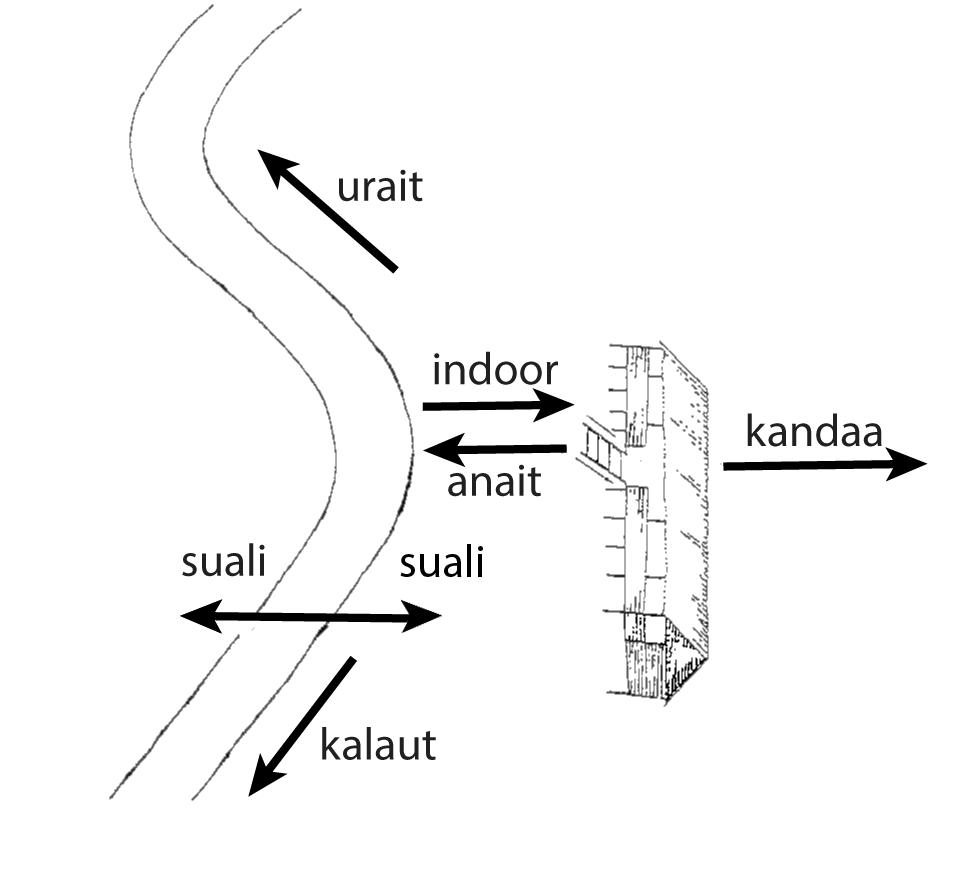
\includegraphics[width=mywidth]{myfig}
    \caption{My Caption}
    \label{fig:my_label}
\end{figure}
\end{lstlisting}}



\begin{figure}[h]
    \centering
    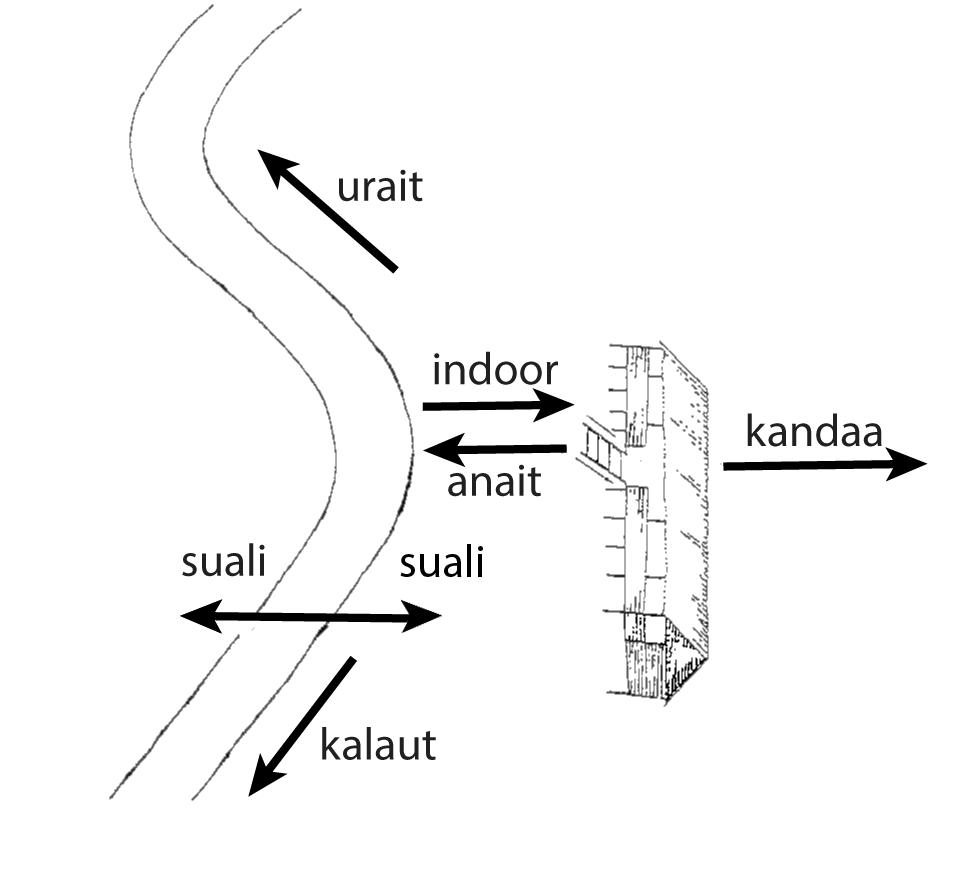
\includegraphics[width=0.5\textwidth]{myfig}
    \caption{Embaloh riverine directional terms \citep[after][70]{adelaar1997}.}
    \label{fig:embaloh}
\end{figure}



\chapter{Analysis}\label{chap:analysis}
\section{Reasons not to use \LaTeX}
{\LaTeX} is a typesetting tool. It's purpose is to provide pretty formatted documents. As such, it is a very appropriate tool for dissertation writing. Dissertations are single-authored documents, and while the Graduate Division may review the document to ensure that it meets university formatting guidelines, the author is typically responsible for achieving that formatting. The onus is on the author to take care of the creation of a table of contents, formatting  and numbering of linguistic examples,  internal cross-referencing, management bibliographic references---and many other tasks which would typically be handled by a publisher. With no publisher (and editor!) to intervene, {\LaTeX} fills the gap. For shorter documents, similar results can be achieved using word processors such as Microsoft Word. However, the use of word processors does not scale well for typesetting large documents such as dissertations.

\subsection{{\LaTeX} for journal publications}
Many linguistic publishers still make use of proprietary typesetting tools and workflows which require authors to submit final copies of manuscripts as a word processing document (often MS Word or RTF). While these publishers may permit authors to submit manuscripts for review as PDF's, once the review process is complete and final edits have been approved, they will request a word processing version of the document. Typically, this version will be required to have minimal formatting, e.g., no automatic numbering, interlinear examples tab-separated or in tables, etc.  This version will then be used by the publisher to create the final layout. The problem for {\LaTeX} users is that there is no reliable method to export from {\LaTeX} to a word processing format such as MS Word. It is possible to use Adobe Acrobat to export the \LaTeX-generated pdf to .docx, but extensive cleanup of the exported document may be required. 

Increasingly, many publishers are using {\LaTeX} for their in-house typesetting, and these publishers may accept and even encourage submissions in {\LaTeX} (with a pdf for review). Moreover, the move toward open-access publishing has resulted in publishers placing more of the type-setting burden on authors. For example, Language Sciences Press strongly encourages {\LaTeX} submissions. Bottom line: check with the publisher before you get too far along in the writing process. If the publisher requires submission in a word processing format, then you may find it easier to use a word processor to write your article. Use the right tool for the job.

\subsection{Co-authoring and collaboration with \LaTeX}
Collaboration is the norm these days, both within Linguistics and across the sciences more broadly.
While the dissertation is a single-authored document, it is likely that many if not most of your publications will be co-authored. 
The emergence of online {\LaTeX} compilers such as \href{http:overleaf.com}{Overleaf} has made it much easier to collaborate---even incorporating commenting and tracked changes. 
However, co-authoring with {\LaTeX} generally requires all authors to be proficient in the use of {\LaTeX}.  If one or more authors are new to {\LaTeX}, then depending on the length of the collaboration, bringing them up to speed may be impractical. The team may find it easier to adopt a common word processing platform instead.

One occasionally encounters the reverse scenario, where one or more authors profess an inability to use a word processor and insist on using \LaTeX. I find that such claims typically a philosophical stance rather than statements about ability. In general, it is easier for a {\LaTeX} user to learn to use a word processor than the other way around. However, there may be ulterior motives, such as a word processor user expressing a desire to learn \LaTeX. In this case the co-authoring process may represent an excellent learning opportunity.  Bottom line: adopt a writing tool which will work for all members of the team. In many cases this tool will not be \LaTeX. Co-authorship requires compromise. 


\section{Citations and bibliography management}\label{sec:citations}
\LaTeX\ interfaces with very powerful bibliographic management tools. See the file references.bib for an idea of how citations are stored. There are many tools available for managing citations, such as \href{https://bibdesk.sourceforge.io/}{BibDesk}. You can also export from common tools such as Zotero.  There are many examples of the use of citations within this document.

Next to the formatting of linguistic examples, the ability to efficiently manage references is probably the most powerful reason to use {\LaTeX} for writing your dissertation. 
% \chapter{Conclusion}\label{chap:conclusion}

\blindtext


\chapter*{References}\addcontentsline{toc}{chapter}{References}
\bibliographystyle{glossa}
\bibliography{references}

\chapter*{Appendix A}\label{chap:appendix}\addcontentsline{toc}{chapter}{Appendix A}

\chapter*{Appendix B}\label{chap:appendix}\addcontentsline{toc}{chapter}{Appendix B}



\end{document}
